    \section{Teknisk beskrivning}
\label{tekbeskrivning}

%Genom att det fyller i de kompetensluckor som en typisk läsare har,
%underlättar bakgrundstexten läsandet av konstruktionsavsnitten. Precis
%som avsnitten Syfte och Mål ovan kan detta avsnitt med fördel
%återanvändas i den slutgiltiga projektrapporten. När det gäller
%projektplanen för DAT290 beskrivs här bakgrunden till projektet vad
%gäller tillämpningen, dess sammanhang och de tekniska förutsättningar
%som råder. För att beskriva tillämpningen och dess sammanhang behöver ni
%förklara hur system av den typen som ska konstrueras här fungerar i
%största allmänhet.

%Men vem är den typiska läsaren? Man får förutsätta att läsaren har en
%viss teknisk kompetens, annars blir bakgrundsavsnittet alltför långt.
%Denna gränsdragning (“hur elementärt ska jag förklara vad jag gör?”)
%upplevs som ett svårt moment när man som student börjar skriva tekniska
%rapporter. En användbar regel är att vi utgår från att läsaren har, i
%stort sett, samma utbildning som rapportskribenten, men saknar
%specialistkunskap om projektets tillämpning.

Denna sektion beskriver hur projektets delsystem implementerades utefter systemets design och krav.
Systemet är uppdelat i moduler enligt figur \ref{fig:systemoversikt}. Nedanstående rubriker går in i mer detalj om respektive modul.



%\subsubsection{Nätverkslagret}
%\label{sec:nätverkslagret}
%Nätverkslaget tar hand om kommunikationen mellan enheterna, vilket  sker %över en CAN-buss (Controller Area Network). Alla enheter som använder sig %av CAN-bussen skickar och tar emot meddelanden med hjälp av protokoll som %utvecklades under projektets gång. Kommunikationen sker igenom %centralenheten.
%\newline\newline
%För att åstadkomma flexibilitet och modularitet skrevs ett CAN-bibliotek. %Biblioteket innehåller funktioner som skickar samt hanterar mottagande av %CAN-meddelanden. Biblioteket kan användas på alla periferienheter men %funktioner för att hantera enhetsspecifika meddelanden måste manuellt %imlementeras. 
%\newline\newline
%Ett CAN-meddelande består av 4 bytes av data samt en 8 bytes buffert för %resterande data. Det första byte-segmentet berättar huruvida meddelandet %kommer från eller till centralenheten, den andra berättar meddelandets %typ, den tredje berättar ID:et på noden som skickat meddelandet och den %fjärde talar om längden på meddelandets databuffert(i bytes).
%\newline\newline
\subsection{Nätverkslagret}
\label{sec:nätverkslagret}
För att standardisera hur meddelanden skickas och tas emot skrevs ett CAN-bibliotek. Biblioteket innehåller funktioner som skickar samt hanterar mottagande av CAN-meddelanden. Biblioteket kan användas på alla periferienheter men funktioner för att hantera enhetsspecifika meddelanden måste manuellt implementeras.
\newline\newline


\begin{figure}[h]
    \centering
    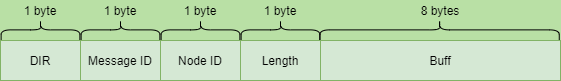
\includegraphics[scale=0.6]{dokumentation/projektrapport/IMAGES/can_msg_struct.png}
    \caption{Structen som representerar ett CAN-meddelande.}
    \label{fig:can_msg_struct}
\end{figure}

I koden skapades också en struct som representerade ett CAN-meddelande. Denna struct bestod av fyra bytes av riktnings- och destinationsdata samt längd på databufferten. Efter dessa finns det en buffert på åtta bytes för resterande data. Det första byte-segmentet beskriver huruvida meddelandet kommer från eller till centralenheten, det andra beskriver meddelandets typ, och det tredje representerar CAN-ramens ID och det fjärde talar om längden på meddelandets databuffert(i bytes). En visualisering av structen finns i figur \ref{fig:can_msg_struct}.
\newline\newline
Meddelandetyperna, som nämns i tabell \ref{tab:msg_types}, har definierats som konstanta heltalsvärden i koden. Prioriteringen av meddelandetyperna räknas ut genom en summering av ID för noden i meddelandet och ID för meddelandetypen. 



\subsection{Centralenhetens logik och datahantering}
\label{sec:centrallogik}
%%Fixa finare intro
När systemet startas aktiverar centralenheten en ''uppstarts-fas''. Den inleds med att centralenheten skickar ut ett ping-meddelande till alla enheter. När centralenheten märker att den har fått ett svar extraherar den informationen från meddelandet, skapar en datarepresentation av modulen, och lägger in den i en lista. Informationen som läggs in är bland annat modulens unika ''id'' och modulens typ, etc. Om en modul inte rapporterar inom tidsramen för uppstarts-fasen läggs den inte in i listan. Då ignoreras följande meddelanden från denna modul.
\newline \newline
Efter uppstarsfasen är klar skickar centralenheten ping-meddelanden till alla enheter varje sekund. Om en av enheterna inte hinner svara innan nästa meddelande skickas, sänder centralenheten en larmsignal till alla larmenheter. En larmsignal skickas också om centralenheten märker att dörrenheten larmar, och dörren i fråga är aktiverad.
\newline \newline
För att lagra information gällande modulerna använder sig centralenheten av en speciellt utformad datatyp. Datatypen och dess fält beskrivs i figur \ref{fig:module}. 
\begin{figure}[h]
    \centering
    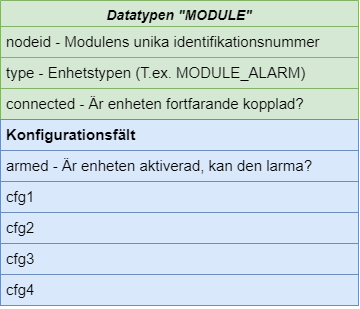
\includegraphics[scale=0.5]{dokumentation/projektrapport/IMAGES/diag_module.png}
    \caption{Datatypen ''MODULE'', gröna fält är konfigurationsfält.}
    \label{fig:module}
\end{figure}
\label{sec:centralenhetDL}
\begin{figure}[h]
    \centering
    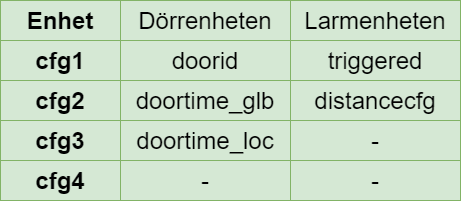
\includegraphics[scale=0.5]{dokumentation/projektrapport/IMAGES/cfg_fields.png}
    \caption{Modulernas konfigurationsfält, '-' betyder att fältets värde är odefinerat.}
    \label{fig:cfg}
\end{figure}

Konfigurationsfälten beskriver modulens nuvarande inställningar. Det första fältet beskriver om enheten är larmad eller inte, och resten beror på vilken modultyp enheten är. I figur \ref{fig:cfg} beskrivs det vad ''cfg1'' till ''cfg4'' representerar för detta projektets moduler. \\ \\
Dörrenhetens ''doorid'' anger hur många dörrar som dörrenheten är konfigurerad för. De följande fälten, localtime och globaltime är hur länge en dörr kan vara öppen innan dörrenheten slår lokalt respektive globalt larm. 
När det gäller larmenheten är ''cfg1'' ''triggered'', och beskriver om larmet är triggat. Det andra fältet representerar vilket avstånd som avståndsmätaren ska larma vid. Värdet i detta fält kan vara från 1-255, mätt i centimeter. %maxavståndet för sensorn (se \ref{sec:sensortyper}). Resten av fälten (''cfg3'', ''cfg4'') lämnas %tomma för båda enheterna. 

\subsection{Centralenhetens IO}
\label{sec:centralenhetIO}

%Centralenhetens knappsats används för att ta emot en kod användaren har slagit in. Koden vidarebefordras sedan till centralenheten som verifierar koden och stänger av. USART används för att ge kommandon och konfigurera moduler. USART används även som en utport där programmet kan skriva ut statusmeddelande för att simplifiera debugging-processen.
%\newline\newline
%Eftersom centralenheten tar emot information från flera olika källor är det viktigt att funktionerna som hanterar IO från knappsatsen och USART kan löpa kontinuerligt.  

%ett att alla inmatningar kan registreras och skickas vidare på kort tid används ett buffertsystem för båda enheterna

%Centralenheten kräver ett kontinuerligt system, där ingen funktion avbryter programmet (\ref{sec:centralenhetIODE})..

Centralenhetens IO-enheter knappsatsen och USART har sitt eget buffertsystem. Ett buffertsystem hanterar en inmatning ifrån USART och knappsatsen genom att lagra endast en bokstav eller siffra i bufferten. Programmet går sedan vidare för att kolla om det finns indata från andra källor. Därefter kan inmatningen fortsätta, vilket tillåter programmet att köra alla sina funktioner kontinuerligt. \\

Konfiguration av programmet sker via USART-kommandon som konfigurerar modulernas register (se \ref{sec:centrallogik} figur \ref{fig:cfg} för lista av alla register). Ett kommando har strukturen [funktion] och potentiellt [modul ID], där funktion står för följande funktioner: 
\begin{itemize}
    \item arm - Armerar en modul genom att sätta modulens armed register till ett givet en modul-ID.
    \item disarm - Desarmerar en modul genom att sätta modulens armed register till noll givet en modul-ID.
    \item status - Returnerar all information om en modul vilket inkluderar en lista över modulens register och deras innehåll givet en modul ID.
    \item config - Tillåter användare att konfigurera en moduls register givet en modul-ID. Detta sker genom att efter användaren skrivit in ''config [Modul-ID]" uppmanas de att skriva in information till varje register i modulen med kommatecken emellan, t.ex ''0,15'' för en larmenhet. 
    \item printlist - Returnerar en lista av alla kopplade modulers typ och ID.
    \item help - Returnerar en lista av alla möjliga kommandon i USART och deras parametrar.
\end{itemize}

Processen från en inmatning till ett exekverat kommando börjar med att användaren skriver in bokstäver i USART vilka lagras i bufferten. När användaren trycker ''retur'' skickas de bokstäver som har lagrats i bufferten vidare till en funktion som bearbetar inmatningen. På grund av kommando strukturen delas inmatningen upp i två delar, ett ord ''funktion'' och ett ''modul-ID''. Det inskrivna ordet jämförs sedan med en lista med möjliga kommandon. Om det finns i listan körs det kommandot med hjälp av modul-ID, annars avbryts kommandot. \\

Vid larm aktiveras knappsatsen där användaren kan skriva in koden. Inmatningen lagras i knappsatsens buffer tills lika många siffror som längden på lösenordet har tagits emot. Därefter verifieras koden och om rätt kod har angetts avlarmas systemet. Användaren får upprepade försök att skriva in rätt kod. Lösenordets inmatning kan återställas genom att trycka på C (clear) på knappsatsen.

\subsection{Dörrenheten} 
\label{sec:dörrenheten}
När dörrenheten kopplas upp för första gången körs ett antal initierande funktioner. En av dem aktiverar SysTick som används för tidsavläsning genom att ett värde ökas varje gång SysTick ger avbrott. Systick ger avbrott varje givet antal klockcykler, vilket anges i initialiseringen. När en dörr med larm aktiverat öppnas sätts den dåvarande tiden som en tidsstämpel. Programmet granskar därefter med jämna mellanrum om dörren varit öppen längre än tillåtet och larmar då lokalt eller globalt beroende på konfigurationen. Om dörren stängts innan tidsgränsen nåtts nollställs tidsstämpeln och eventuellt lokalt larm stängs av. Ett globalt larm som gått måste stängas av från centralenheten.
\newline\newline
För att klara av att hålla reda på hurvida dörrarna är öppna eller stängda använder den en uppsättning dörrsensorer som ger information om dörren är öppen eller stängd. Dörrenheten håller reda på hur länge sedan sensorns krets bröts och beroende på det utlöser den passande larm.
\newline\newline
En struct för dörrar har skapats. Dörrstructen innehåller följande data.
\begin{itemize}
    \item Dörrens ID
    \item Vilken GPIO-pinne dörren är kopplad till
    \item Om den är öppen eller stängd
    \item Röd diodstatus
    \item Larmfunktion på-/avslagen
    \item Tidsgräns för globalt larm
    \item Tidsgräns för lokalt larm
    \item Tidsstämpel
\end{itemize}


Upp till åtta dörrar stöds. För fler än åtta dörrar behövs flera dörrenheter. När programmet startas initieras alla åtta dörrar med standardvärden. När centralenheten sedan skickar det första konfigurationsmeddelandet (se \ref{sec:centralenhetDL}) konfigureras alla dörrar upp till den givna dörren efter inställningarna i meddelandet. Alla dörrar som då inte konfigureras tas då bort ur systemet.
\subsection{Larmenheten}
\label{sec:larmenhet}
Larmenhetens inportar är konfigurerade till pinnarna GPIOE0-15. Därför kopplas avståndssensorns ekosignal samt vibrationssensorns utsignal via dessa pinnar. GPIOD0-15 är reserverade som utportar, de kopplas till avståndssensorns inport och lokala larmets lampor.
\newline\newline
Larmenhetens programlogik är uppbyggd för att lyssna på sensorerna och centralenheten kontinuerligt och märka om ett larm måste utlösas. Vibrationssensorn är direkt kopplad till larmfunktionen i och med att tröskelvärdet  konfigureras analogt. Till skillnad från vibrationssensorn måste programlogiken hantera både avståndssensorns in- och utdata. För att aktivera avståndssensorn skickas en tio mikrosekunders högnivåsignal till sensorns inport  (markerad "Trig"). Ekot mäts därefter och ger en högnivåsignal på utporten (markerad "Echo") proportionell till tiden pulsen färdas (se figur \ref{fig:Sonar}). Tidsintervallet jämförs sedan med värdet “time\_to\_trigger\_sound” som bestäms från det kalibrerade eller konfigurerade värdet från centralenheten. Om tiden som mätts är mindre än “time\_to\_trigger\_sound”, dvs objektet är närmare än det konfigurerade avståndet utlöses larmet.
\begin{figure}[h]
    \centering
    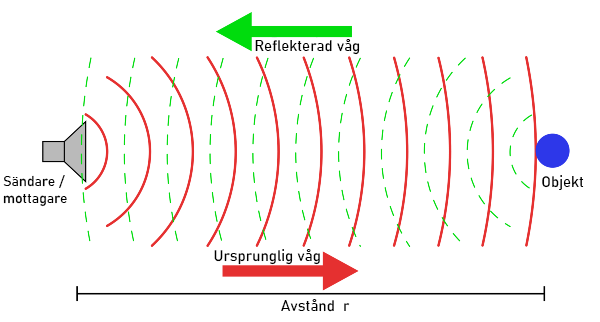
\includegraphics[scale=0.58]{dokumentation/projektrapport/IMAGES/Sonar.png}
    \caption{Avståndssensor. Avståndet räknas ut med: $r = (t * v_{ljud}) / 2$,\newline $t$ = tiden av högnivåsignalen från echo, $v_{ljud}$ = ljudets hastighet (343m/s).}
    \label{fig:Sonar}
\end{figure}
\newline\newline
Utöver detta tänder larmenheten en varningslampa så fort något närmar sig avståndssensorn. Avståndet för att tända lampan är dubbelt så långt som det konfigurerade värdet från centralenheten.
\newline\newline
Ifall larmenheten mottager ett meddelande från centralenheten hanteras det omedelbart med ett avbrott. Avbrottshanteraren för vidare meddelandet till en hanteringsfunktion beroende på vilken typ av meddelande det är. De meddelandetyper som hanteras är konfigureringsmeddelanden, meddelanden för att växla av/på larmet och pingmeddelanden. Ett konfigureringsmeddelande innehåller:\newline
\begin{itemize}
    \item En byte som bestämmer om larmet ska vara armed (se figur \ref{fig:module}).
    \item En byte som bestämmer om larmet ska slå larm/sluta slå larm direkt (se figur \ref{fig:cfg}).
    \item En byte som antingen kan:
    \begin{itemize}
        \item Ge en order att kalibrera sensorn efter de objekt som finns framför den i nuläget, detta sker när byten är noll.
        \item Ge ett bestämt avstånd som avståndssensorn ska konfigureras efter.
    \end{itemize}
\end{itemize}


När ett pingmeddelande är mottages skickas ett svarsmeddelande tillbaka. Dessutom sparar funktionen tidspunkten då larmenheten senast tog emot ett pingmeddelande. Eftersom larmenheten är den enda enheten i systemet som kan producera ett larm måste det finnas någon motåtgärd om larmenheten skulle kopplas ifrån systemet. Den motåtgärden består av att om larmenheten slutar tar emot ping-meddelanden från centralenheten i åtminstone en sekund larmar enheten automatiskt, dock är det värt att notera att centralenheten inte får ett meddelande om larmet är igång.


\subsection{Störenheten}
\label{sec:störenhet}
Störenheten har förmågan att skicka både korrekt strukturerade CAN-meddelanden eller slumpade datasträngar. Mängden data och frekvensen på meddelanden är inte konfigurerbara genom systemet utan måste föranpassas i koden. Detta anses acceptabelt då enheten är enkel och endast används när tester utförs på systemet. 


\subsection{Användning}
\label{sec:användning}
Programmet startar med en ''uppstartsfas'', där alla moduler kopplas till programmet automatiskt (se \ref{sec:centralenhetenDE}). Alla enheter är initialt icke-armerade, vilket betyder att de inte kan användas. För att armera modulen behövs USART-kommandon användas (se \ref{sec:centralenhetIO}). En användare som aldrig har använt programmet tidigare kan t.ex först skriva ''help'' för att se möjliga kommandon. Sedan kan användaren skriva ''printlist'' för att se vilka moduler är kopplade och deras ID. Slutligen kan användaren börja konfigurera eller armera/disarmera modulerna med ''arm/disarm [modul-ID]'' eller ''config [modul-ID]'', där [module-ID] är en av ID värdena från printlist. \\

När ett lokalt larm utlöses tänds en lampa, och på dörrenheten startas en timer. För att larma av innan ett globalt larm utlöses behöver användaren skriva in rätt pin-kod med knappsatsen. Om användaren skriver fel får den återkoppling via USART, och får ett nytt försök. Om det skrivs in mindre än fyra siffror kan användaren fortfarande börja om genom att trycka på knappen ''C'' (clear). \\

För att ansluta dörrar till en dörrenhet skall dörrsensorer kopplas till GPIOE 0-7, röda dioder till GPIOD 0-7 och gröna dioder till GPIOD 8-15. Om färre dörrar än åtta vill anslutas skall dessa anslutas till de lägra pinnarna. Sedan konfigureras antalet dörrar genom USART. Om t.ex två dörrar ska anslutas kopplas två dörresensorer till GPIOE 0-1, Två röda dioder kopplas till GPIOD 0-1 och två gröna dioder kopplas till GPIOD 8-9.
\iffalse
För att konkretisera en struktur som ett datorsystem underlättar det
ofta att rita en figur, till exempel ett blockschema, över systemet som
man tänker sig att implementera. I detta avsnitt beskriver ni
översiktligt systemet, lämpligen genom en (eller flera) figur(er). Se
till att hänvisa till figuren från texten och att använda en rubrik för
figuren. Eftersom systemet är ganska komplext behöver ni tänka igenom
vilken detaljrikedom systemöversikten ska ha; dels känner ni ännu inte
till detaljer eftersom konstruktionsarbetet inte påbörjats, dels skulle
inte alla detaljer få plats i en figur över systemet.

I och med att det finns ett grundsystem till vilket man kan lägga
kompletteringar behöver era val av kompletteringar beskrivas
översiktligt. Om ni avser att arbeta med egendefinierade kompletteringar
krävs en mer detaljerad beskrivning än om ni använder kompletteringar
som beskrivs i projektdirektivet.

Under projektets genomförande kommer ni att få anledning att revidera
figuren över systemet. Att ta fram den ultimata figuren över det
slutliga systemet är varken möjligt eller önskvärt under
planeringsfasen, utan det är framförallt processen med att ta fram
figuren som är viktig eftersom denna process hjälper gruppen att
fokusera tänkandet, att skapa gemensamma tekniska ramar och att rensa
bort (en del) tekniska oklarheter.
\fi